
\chapter{Self-calibration for Coded Illumination Systems}

\section{Introduction}
Quantitative Phase Imaging (QPI) enables label-free and stain-free imaging of biological samples \emph{in vitro} through the recovery of the complete complex-field (absorption and phase). Differential Phase Contrast (DPC)~\cite{Hamilton1984a,Tian14} is a partially coherent phase contrast technique that can recover quantitative phase~\cite{mehta2009quantitative,tian2015quantitative} from captured images that each use different half-circle source patterns. Since phase information is encoded in Fourier asymmetry, these images can be used to recover phase using a single-step deconvolution process~\cite{mehta2009quantitative,tian2015quantitative}, assuming a linearized model. DPC recovers both amplitude and phase with resolution up to the incoherent resolution limit ($2\times$ better than coherent methods). Practically, the illumination coding can be done with a low-cost LED array~\cite{Tian14,zijiMulti,tian2015quantitative}. At least two complementary source patterns are required, but generally 4 patterns (top, bottom, left, right half-circles) are used to avoid missing spatial frequencies.

Aberration recovery using an LED array has previously been used for the deconvolution of fluorescence images~\cite{Ou:14}, but this method requires many images since it is based on Fourier Ptychography. In this work, we present a method of recovering the same aberration function as in~\cite{Ou:14}, and the complex-field, using just 4 images. By segmenting our field-of-view prior to reconstruction, we are able to recover spatially-variant aberration functions. While our DPC-based blind-deconvolution method is inherently nonlinear and cannot be guaranteed to converge to a global minimum, we show experimentally that it is in practice accurate and robust.

\section{Differential Phase Contrast}
DPC employs a linearized forward model to describe the intensity images that result from a given complex-field. The linearization can be a result of a weak phase assumption on the sample's complex-field, ignoring higher order (nonlinear) terms in the Taylor expansion of the complex-field, $\vec{E} = e^{\mathrm{i}\phi -\mu} \approx 1-\mu + \mathrm{i}\phi$.
Under the same approximation, the Weak Object Transfer Functions (WOTFs) for absorption ($\tilde{H}_{\mu}$) and phase ($\tilde{H}_{\phi}$) can be derived~\cite{Claus2015, tian2015quantitative, Hamilton1984a} to linearly related to intensity measurements:

\begin{equation}
	I(\vec{r}) = I_{0} +H_{\mu}(\vec{r}) \otimes \mu(\vec{r}) + \mathrm{i}\cdot H_{\phi}(\vec{r}) \otimes \phi(\vec{r}).
	\label{eq:two}
\end{equation}

\noindent Here, $\vec{r}$ represents 2D real-space coordinates, $I$ is the intensity measurement, $I_0$ is the background signal, and $\otimes$ denotes convolution. Given a known source ($S$), and pupil function ($P$) whose bandwidth is set by the objective numerical aperture (NA) and wavelength ($\lambda$), the WOTFs are~\cite{Claus2015,tian2015quantitative}:

\begin{equation}\label{WOTFre}
\tilde{H}_{\mu}(\vec{k}) = P(\vec{k}) \star (P(\vec{k})\cdot S(-\vec{k}))+ (P(\vec{k}) \cdot S(-\vec{k})) \star P(\vec{k})
\end{equation}

\begin{equation}\label{WOTFim}
\tilde{H}_{\phi} (\vec{k}) = P(\vec{k}) \star (P(\vec{k})\cdot S(-\vec{k}))- (P(\vec{k}) \cdot S(-\vec{k})) \star P(\vec{k}),
\end{equation}

\begin{figure}
\centering
\includegraphics[width=0.82\textwidth]{fig_dpc_cal_system.pdf}
\caption{\label{fig:system}
System schematic for Differential Phase Contrast (DPC) microscopy with embedded pupil recovery for aberration correction. Four intensity images are captured with different source shapes.}
\end{figure}

\noindent In both equations, $\tilde{\cdot}$ is Fourier transform, $\vec{k}$ represents 2D spatial frequency coordinates, and $\star$ denotes cross-correlation. The inverse problem~\cite{tian2015quantitative,Claus2015} is linear and can be solved with a one-step deconvolution (e.g. Wiener deconvolution~\cite{HayesDSP}) or by an iterative algorithm (e.g. gradient descent). While previous DPC algorithms~\cite{tian2015quantitative} required four images for accurate phase and amplitude recovery, we have shown~\cite{PhillipsChen17cDPC} that three images are sufficient for QPI. In this work, we exploit this over-determined nature to recover the spatially-variant aberrations (pupil functions) of our optical system.

\section{Pupil Recovery}

Under a spatially coherent source, the pupil function $P$ is defined as the linear filter imposed by the imaging system in the Fourier domain. While the pupil function is generally represented as a 2D complex image, the phase of the pupil usually exists in a sparse Zernike Polynomials basis~\cite{ZERNIKE1934689}, defined as:

\begin{equation}
P(\vec{k}) = \prod_{m,n} e^{\mathrm{i}c_{mn} Z_{mn}}.
\end{equation}

In practice, we find that around 18 coefficients can accurately describe aberrations in our microscope, a major reduction in dimensionality from the Fourier basis. To solve for these coefficients in addition to quantitative phase, we first acquire three images with asymmetric illumination (as in conventional DPC), then add a fourth using single-LED illumination to aid in the recovery of aberrations. In experiments, we accomplish the source coding with an LED array (Fig.~\ref{fig:system}), as in~\cite{tian2015quantitative}. Our modified forward model is $I' = A(c) x(\mu,\phi) $, where $A(c)$ is the forward operator for the formation of intensity images $I'$ composed of the WOTFs with a pupil described by Zernike coefficients $c$, and $x$ is the complex-field containing $\mu$ and $\phi$. The inverse problem is defined as:

\begin{equation}
\label{eq:pupilRecoveryObj}
\begin{aligned}
&\text{min}
& & O(\mu,\phi,c) = \frac{1}{2} ||A(c) x(\mu,\phi) - I'||_2^2 + R(\mu,\phi)  \\
\end{aligned}
\end{equation}

This problem is a blind deconvolution of the pupil coefficients and sample, which is nonlinear. The ideal choice of regularizer $R(\mu,\phi)$ depends on the sample and noise. Here, we use total variation (TV) regularization for denoising. We solve this inverse problem using the alternating minimization algorithm show in algorithm~\ref{alg:pupil}.

\begin{algorithm}
    \caption{Pupil Recovery Algorithm}
    \label{alg:pupil}
    \begin{algorithmic} % The number tells where the line numbering should start
        \Procedure{PupilRecovery}{$\mu,\phi,c$}
            \State $c^1=c_0,\hspace{1pt}\mu^1=\mu_0,\hspace{1pt}\phi^1=\phi_0 $ \Comment{Initialization}
            \For{$k=1$ to MaxIteration}
                \State $\mu^{k+1},\phi^{k+1} = \underset{\mu,\phi }{\text{argmin}} \hspace{3pt} O(\mu,\phi,c^k)$
                \Comment{Optical Field Recovery}
                \State $c^{k+1} = \underset{c}{ \text{argmin}} \hspace{3pt}O(\mu^{k+1},\phi^{k+1},c)$
                \Comment{Pupil Recovery}
                \If{$\frac{| O(\mu^{k+1},\phi^{k+1},c^{k+1})- O(\mu^{k},\phi^{k},c^k)|}{O(\mu^{k+1},\phi^{k+1},c^{k+1})}  < \epsilon$}
                \Comment{Convergence Condition}
                   \State End Iteration
                   \EndIf
            \EndFor
            \State \textbf{return} $\mu,\phi,c$
        \EndProcedure
    \end{algorithmic}
\end{algorithm}

\begin{figure}[H]
\centering
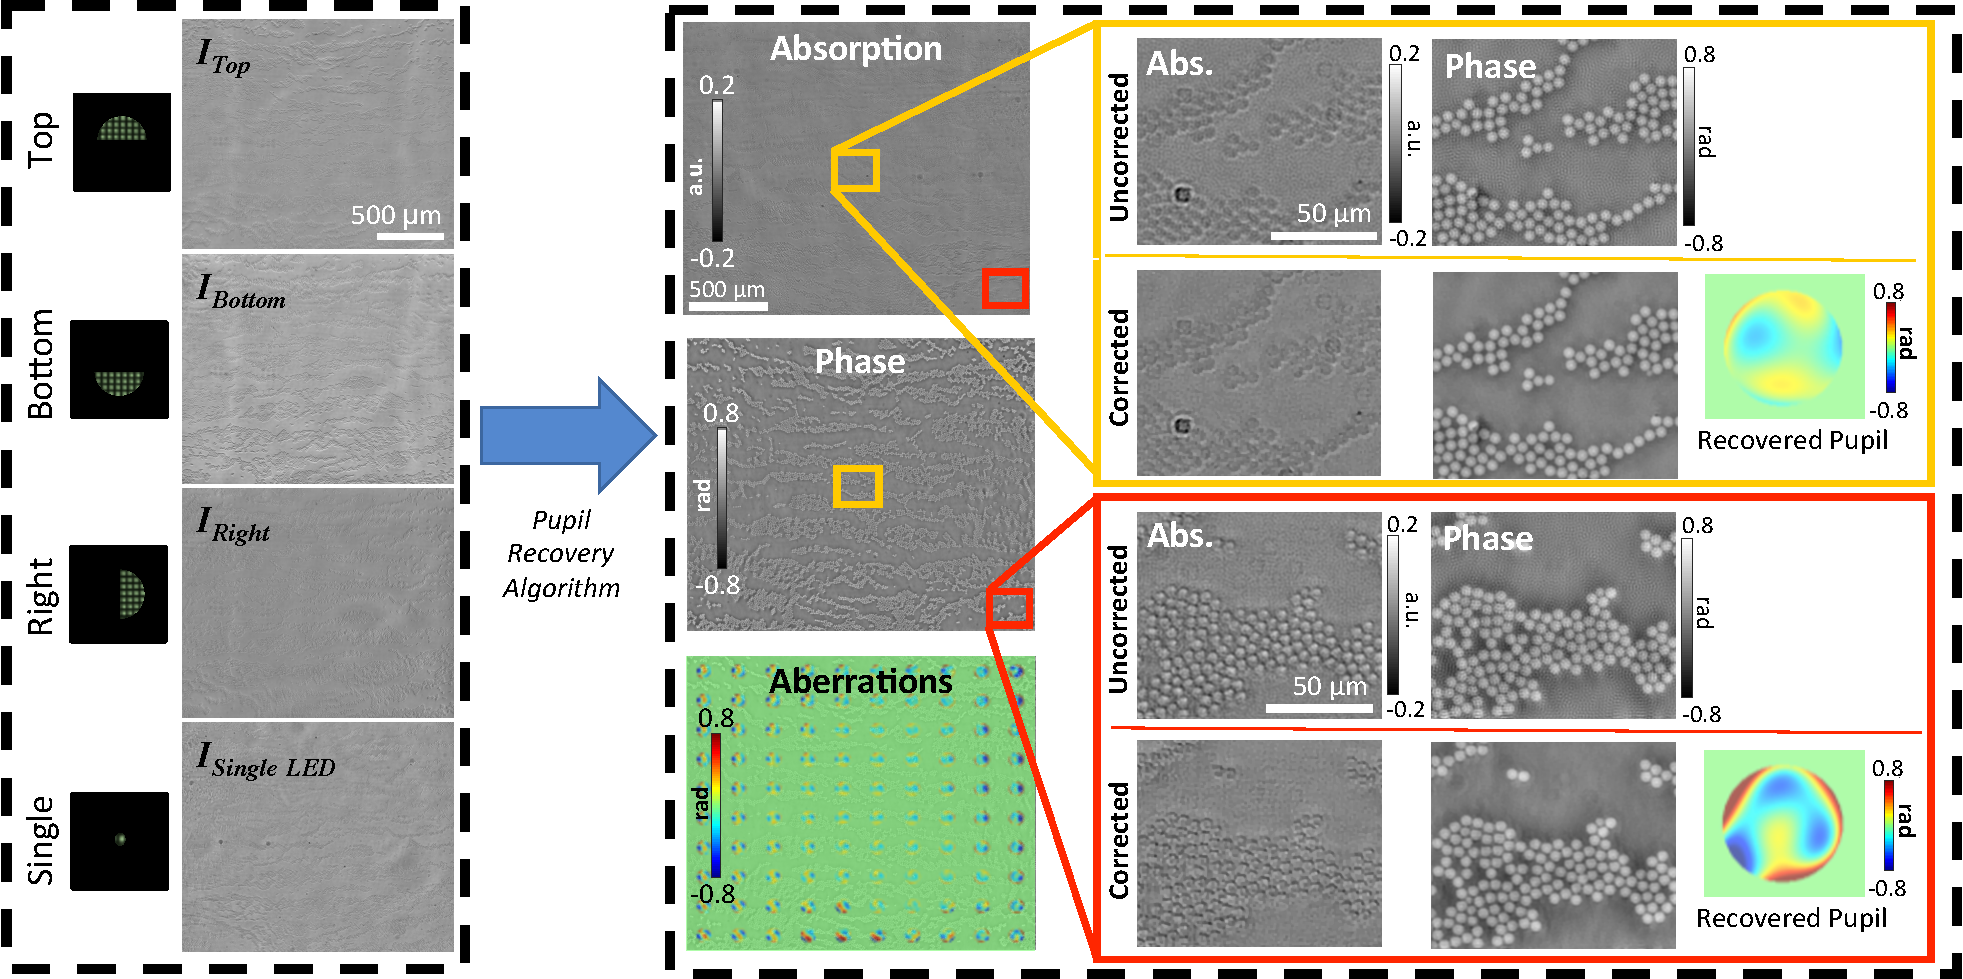
\includegraphics[width=\textwidth]{fig_dpc_cal_result.pdf}
\caption{\label{fig:results}
Experimental results. (Left) Raw data with corresponding source patterns. (Right) Reconstructed absorption, phase, and spatially-variant aberrations are shown for two example locations in the field-of-view, along with a map of the pupil aberration functions across the entire field-of-view.}
\end{figure}

To verify our method experimentally, we used a $4\times$ 0.2NA objective in a Nikon TE300 microscope, which has a wide field of view and therefore significant spatially-variant aberrations. We segment out field into 100 patches and solve for the locally spatially-invariant aberration within each patch. These data were acquired using a monochrome LED array (514nm center wavelength) and a PCO.edge 5.5 sCMOS camera. We acquired four images in total. The results indicate that field-dependent aberrations have a more pronounced affect on amplitude retrieval than phase, but this effect has significant field-dependence at low magnifications. These data show the importance of incorporating pupil retrieval into DPC reconstruction algorithms.
